%REPORT TEMPLATE
%AUTHOR: RUI QU  
%EMAIL: RQU@KTH.SE 

%----------------------------------------------------------------------------------------
%	PACKAGES AND DOCUMENT CONFIGURATIONS
%----------------------------------------------------------------------------------------

\documentclass{article}

%---Basic---
\usepackage{natbib} % Required to change bibliography style to APA
\usepackage{amsmath} % Required for some math elements 
\setlength\parindent{0pt} % Removes all indentation from paragraphs
\usepackage{listings}%Insert code
\usepackage{times} % Uncomment to use the Times New Roman font

%---Table---
\usepackage{multirow}%Table
\usepackage{booktabs}%Table Triple-lines
\usepackage{siunitx} % Provides the \SI{}{} and \si{} command for typesetting SI units

%---Figure---
\usepackage{graphicx} % Required for the inclusion of images
\usepackage{subfigure} % Required for multiple images
\usepackage{float} 

%---Pseudo-code in LaTeX---
\usepackage{minted} %Preference->engine->pdfTeX->Latex  ADD: -shell-escape
\usepackage{xcolor}
\definecolor{bg}{rgb}{0.95,0.95,0.95}

\usepackage{algorithm}
\usepackage{algpseudocode}
\usepackage{amsmath}
\renewcommand{\algorithmicrequire}{\textbf{Input:}}  % Use Input in the format of Algorithm
\renewcommand{\algorithmicensure}{\textbf{Output:}} % Use Output in the format of Algorithm

%---Appendix---
\usepackage{appendix}
\newcommand{\upcite}[1]{\textsuperscript{\textsuperscript{\cite{#1}}}} %Upcite

%----------------------------------------------------------------------------------------
%	DOCUMENT INFORMATION
%----------------------------------------------------------------------------------------

\begin{document}

\title{CS-E5710 Bayesian Data Analysis\\Assignment }                  
%\author{Rui Qu\\rui.qu@aalto.fi}
\maketitle

% If you wish to include an abstract, uncomment the lines below
% \begin{abstract}
% Abstract text
% \end{abstract}

%----------------------------------------------------------------------------------------
%	SECTION 1
%----------------------------------------------------------------------------------------

\section{Stan-model}
The stan model:
\begin{minted}[bgcolor=bg, linenos, fontsize=\footnotesize]{python}  
stan_code = '''
data {
    int<lower=0> n;
    int<lower=0> deaths[n];
    int<lower=0> numb_of_animals[n];
    vector[n] doses;
    vector[2] mu;
    cov_matrix[2] cov_m;
}
parameters {
    vector[2] alpha_beta;
}
model {
    alpha_beta ~ multi_normal(mu, cov_m);
    deaths~binomial_logit(numb_of_animals,alpha_beta[1]
    	+alpha_beta[2]*doses);
}
'''
\end{minted}
Fit the model:
\begin{minted}[bgcolor=bg, linenos, fontsize=\footnotesize]{python}  
sm = pystan.StanModel(model_code=stan_code)
data = dict(
    n=len(number_of_animals),
    deaths=deaths,
    numb_of_animals=number_of_animals,
    doses=doses,
    mu=mean,
    cov_m=cov_matrix,
)
fit = sm.sampling(data=data, chains=10, iter=10000, warmup=1000)
\end{minted}
Outputs:
\begin{minted}[bgcolor=bg, linenos, fontsize=\footnotesize]{bash}  
fit Inference for Stan model: anon_model_40c9b1c0193fdad43559b9bb79df0201.
10 chains, each with iter=10000; warmup=1000; thin=1; 
post-warmup draws per chain=9000, total post-warmup draws=90000.

                mean se_mean     sd   2.5%    25%    50%    75%  97.5%  n_eff   Rhat
alpha_beta[1]   0.97  5.2e-3    0.9  -0.66   0.35   0.93   1.55   2.84  29700    1.0
alpha_beta[2]  10.46    0.03   4.57   3.47   7.03   9.87  13.21  20.93  27236    1.0
\end{minted}

\section{Rhat value}

The Rhat value is $\hat{R}_\alpha=1.0$, $\hat{R}_\beta=1.0$.\\

Interpretation: \\
The potential scale reduction factors is estimated by:
\begin{equation}
\hat{R}=\sqrt{\frac{\hat{var}+(\psi|y)}{W}}
\end{equation}
which declines to 1 as $n\rightarrow \infty$. If the potential scale reduction is high, then we have reason to believe that proceeding with further simulations may improve our inference about the target distribution of the associated scalar estimand. If Rhat-value is not close to 1, it is believed that the testing samples may be not from the same distribution or may not converge. In my test all Rhat-values is 1.0 which means the generated chains converge well.\\

\section{Scatter plot}
\begin{figure}[H]
\centering  
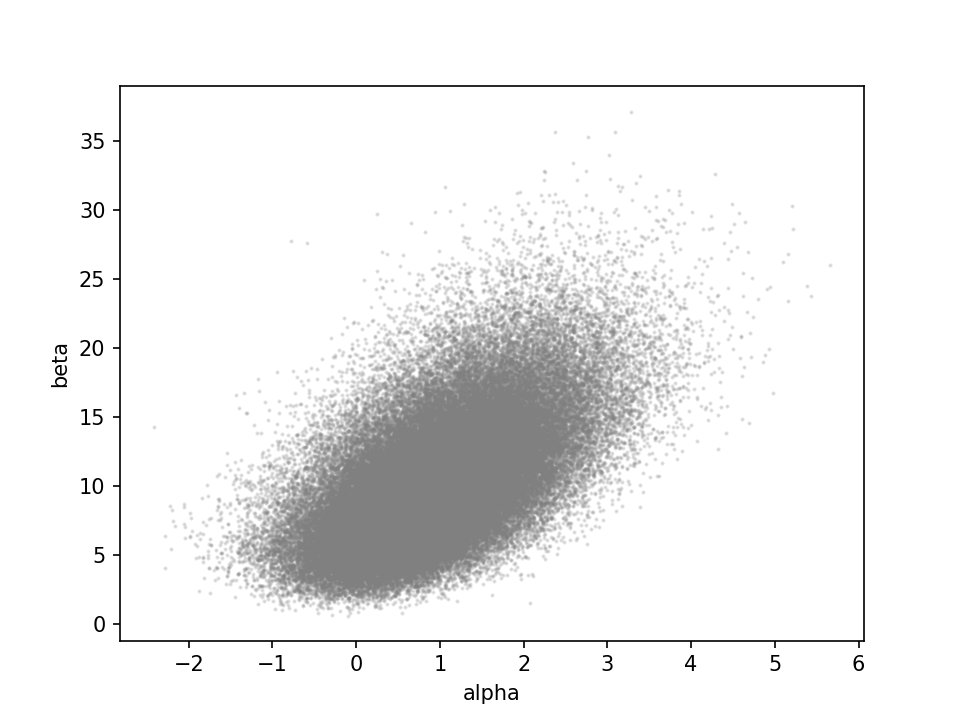
\includegraphics[scale=0.5]{scatter.png}
\caption{Scatter plot}
\label{fig: label}
\end{figure}



\appendix
\section{Code}
\begin{minted}[bgcolor=bg, linenos, fontsize=\footnotesize]{python}  
import matplotlib.pyplot as plt
import numpy as np
import pystan

sigma_a = 2
sigma_b = 10
mu_a = 0
mu_b = 10
cor = 0.5
cov_matrix = np.array([
    [sigma_a**2,                cor * sigma_a * sigma_b],
    [cor * sigma_a * sigma_b,   sigma_b**2]
])
mean = np.array([mu_a, mu_b])

doses = np.array([-0.86, -0.3, -0.05, 0.72])
deaths = np.array([0, 1, 3, 5])
number_of_animals = np.array([5, 5, 5, 5])

stan_code = '''
data {
    int<lower=0> n;
    int<lower=0> deaths[n];
    int<lower=0> numb_of_animals[n];
    vector[n] doses;
    vector[2] mu;
    cov_matrix[2] cov_m;
}
parameters {
    vector[2] alpha_beta;
}
model {
    alpha_beta ~ multi_normal(mu, cov_m);
    deaths~binomial_logit(numb_of_animals,alpha_beta[1]
    	+alpha_beta[2]*doses);
}
'''

sm = pystan.StanModel(model_code=stan_code)
data = dict(
    n=len(number_of_animals),
    deaths=deaths,
    numb_of_animals=number_of_animals,
    doses=doses,
    mu=mean,
    cov_m=cov_matrix,
)
fit = sm.sampling(data=data, chains=10, iter=10000, warmup=1000)
print('fit', fit)

extracted_samples = fit.extract()
samples = extracted_samples['alpha_beta']
plt.scatter(samples[:, 0], samples[:, 1], alpha=0.2, s=1, color='grey')
plt.ylabel('beta')
plt.xlabel('alpha')
plt.savefig('./scatter.png', dpi=150)
\end{minted}



\end{document}